\documentclass{article}
\usepackage[utf8]{inputenc}
\usepackage{graphicx}
\usepackage[margin=2.5cm]{geometry}
\usepackage{eso-pic}
\usepackage{hyperref}
\usepackage{wrapfig}
\usepackage{array}
\usepackage{enumitem}
\AddToShipoutPictureBG{%
    \AtPageLowerLeft{
        % \hspace{1cm}
        
\includegraphics[width=4.5cm]{img/Java-Hutts2.png}
    }
}
\title{System Requirements Specification}
\date{2017}
\def \project{Electronic ID Verification }
\begin{document}

\makeatletter
    \begin{titlepage}
        \begin{center}
            
\includegraphics[width=0.7\linewidth]{img/up.png}\\[4ex]
            {\huge \bfseries \@title }\\[2ex]
            {\LARGE \textbf{Team:} Java the Hutts}\\[2ex]
            {\LARGE \@date}\\[2ex]
            {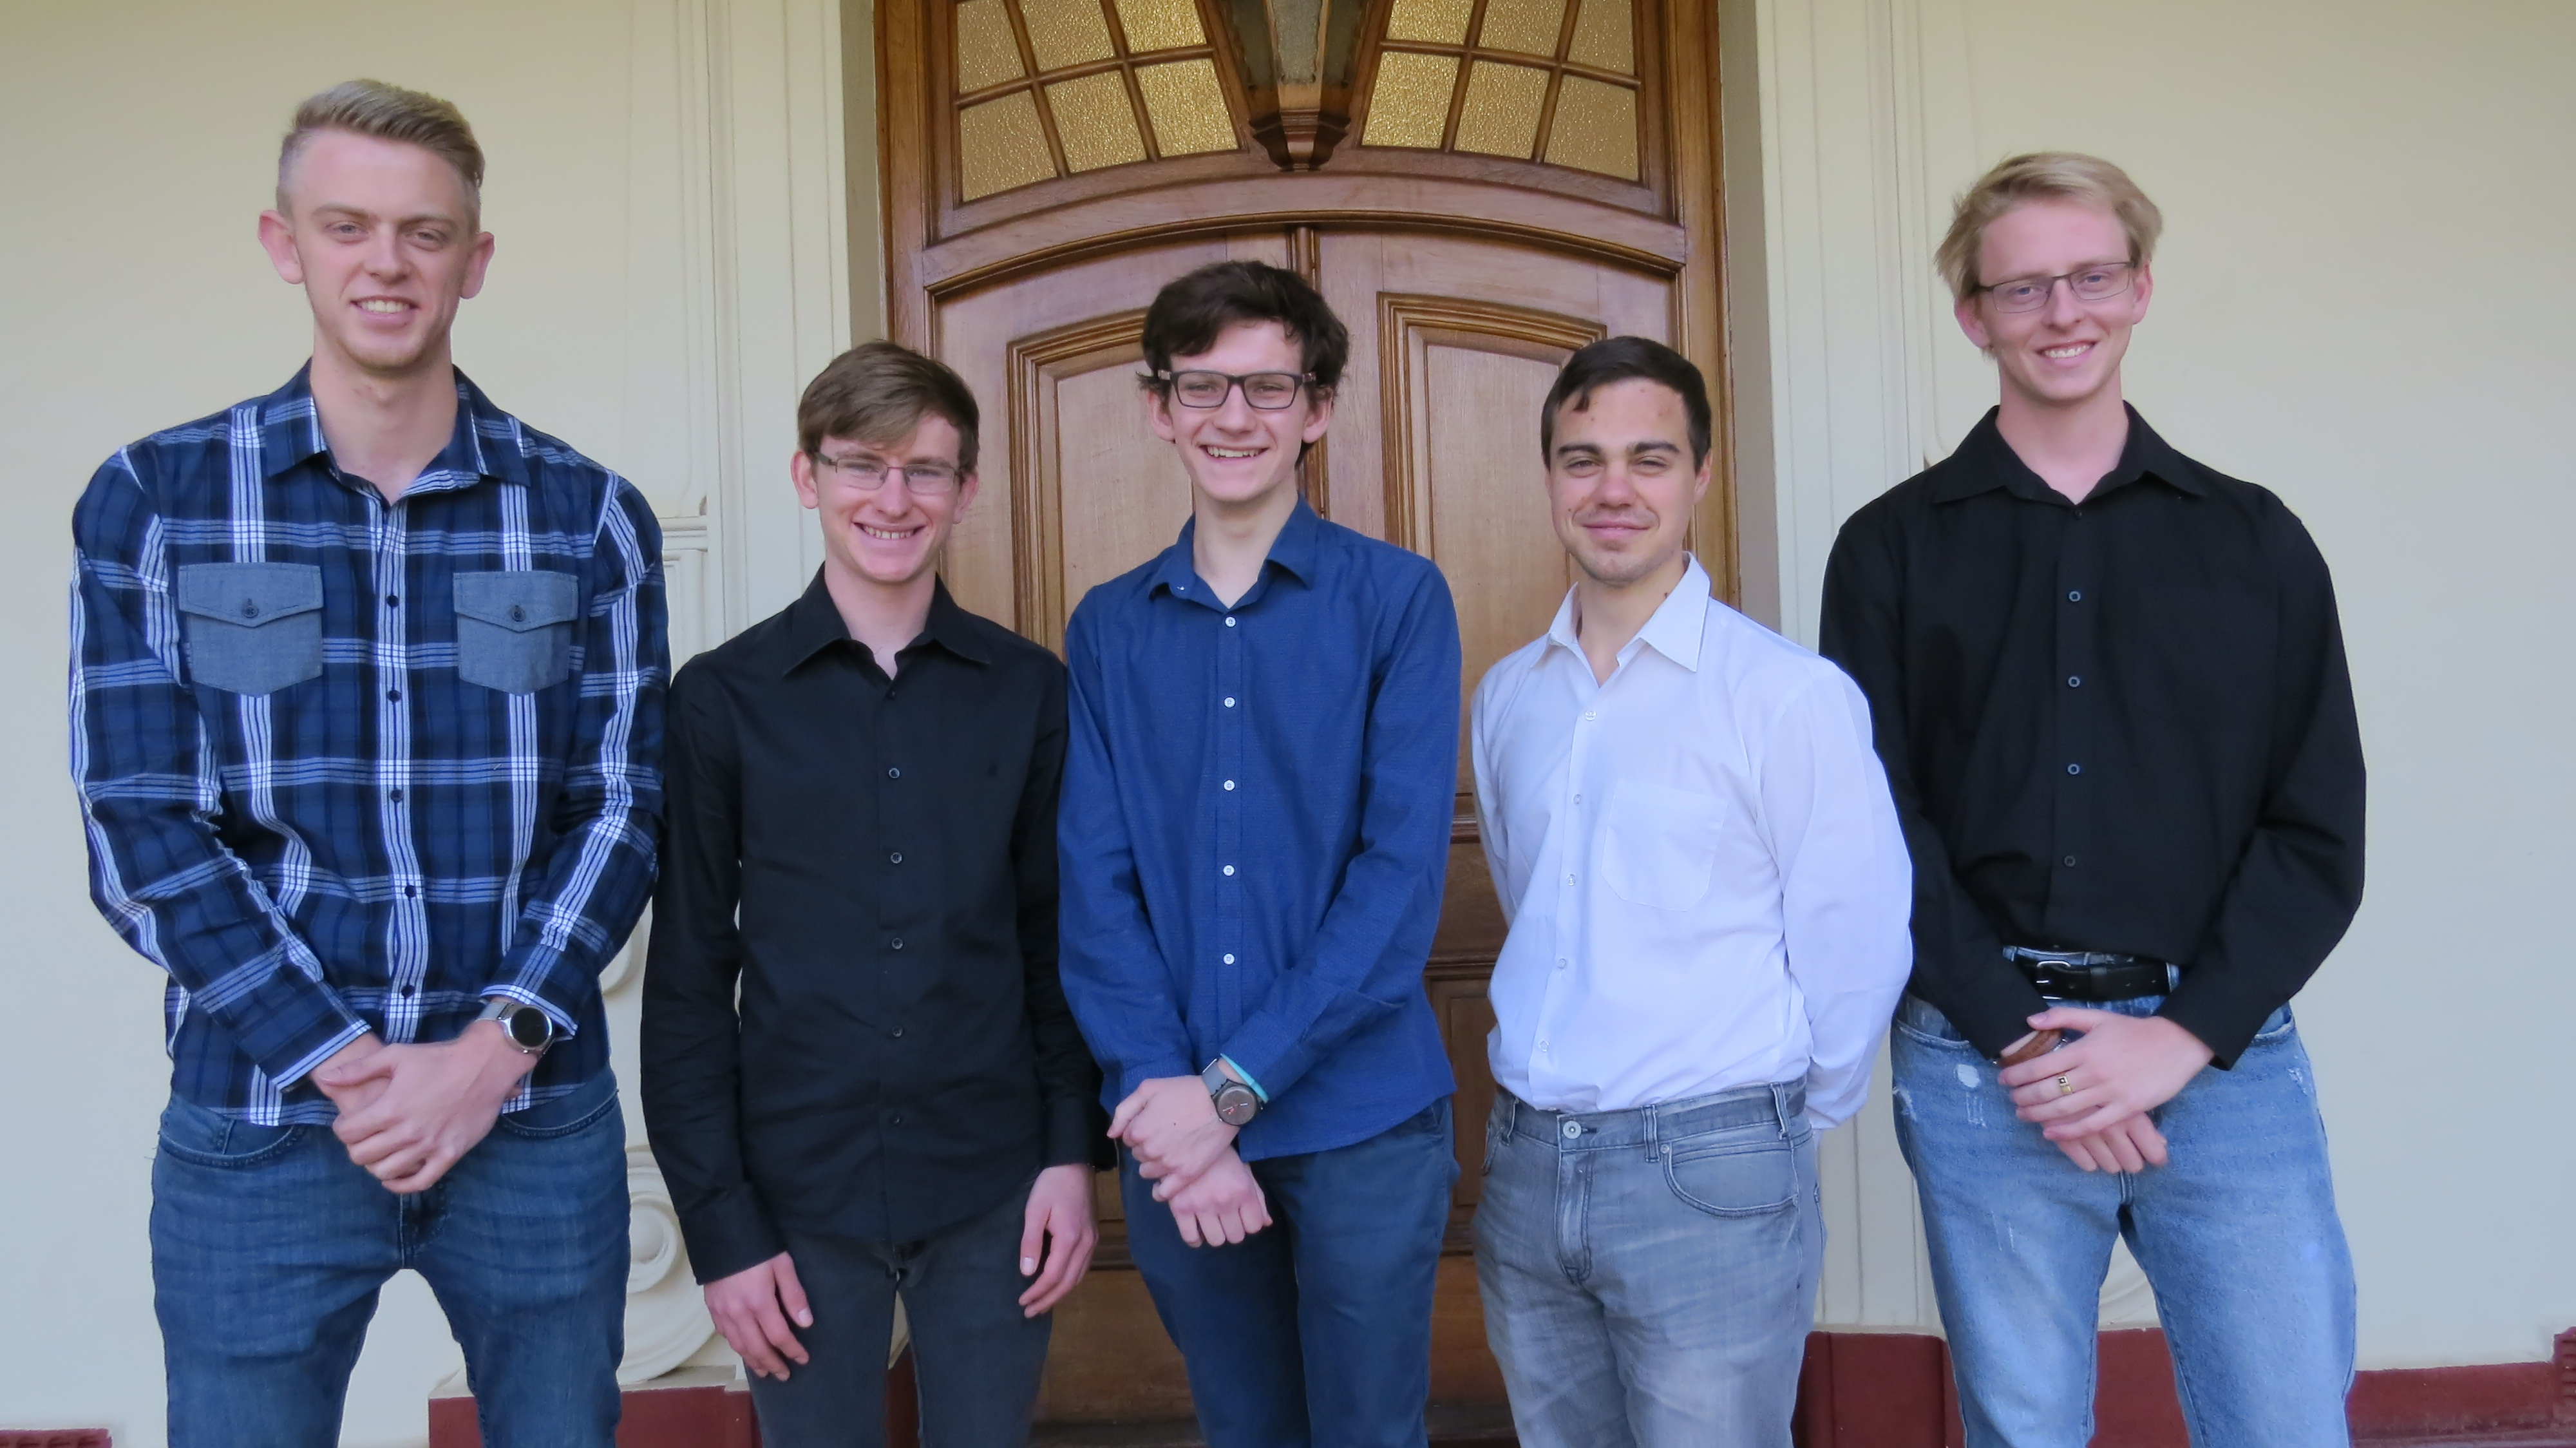
\includegraphics[width=\linewidth]{img/team_photo.jpg}}\\[2ex]
            {\large  Nicolai van Niekerk\\ \texttt{nicvaniek@gmail.com}}\\[2ex]
            {\large  Marno Hermann\\ \texttt{marno@barnton-consulting.co.za}}\\[2ex]
            {\large  Stephan Nell\\ \texttt{nellstephanj@gmail.com}}\\[2ex]
            {\large  Jan-Justin van Tonder\\ \texttt{J.vanTonder@tuks.co.za}}\\[2ex]
            {\large  Andreas Nel\\ \texttt{nel.andreas1@gmail.com}}\\[2ex]
        \end{center}
        
    \end{titlepage}
\makeatother

\cleardoublepage
\thispagestyle{empty}
\tableofcontents
\newpage

\setcounter{page}{1}
	\section{Introduction}\label{sec:intro}
		This chapter aims to give a description, as well as an overview, of the content of this document. Additionally, it will include any terms, abbreviations, acronyms and references used throughout this document.

		\subsection{Purpose}\label{subsec:purpose}
			The purpose of this document is to present the reader with a detailed description of the \project system. It will delve into the purpose and features of the system, the various interfaces of the system, the capabilities of the system, as well as the constraints under which the system must operate. The content of this document is intended for both the various stakeholders and the developers of the \project system.

		\subsection{Scope}\label{subsec:scope}
			The \project is proposed as a standalone system that provides the core functionality of extracting client details from an image of some form of ID, and comparing existing client information with that which was extracted from the image of the ID.

		\subsection{Definitions, Acronyms, and Abbreviations}\label{subsec:daa}
			\begin{table}[h!]
				\centering
				\label{tab: Table 1}
				\begin{tabular}{| m{4cm} | m{12cm} |}
					\hline
                        \textbf{Term} & \textbf{Definition}\\
					\hline
				    	OCR & Optical Character Recognition\\
				    \hline
			            ID & Identification Document\\
					
				    \hline
				        API & A set of functions and procedures that allow the creation of applications which access the features or data of an operating system, application, or other service. \\
				    \hline
				        Linux &  A Unix-like computer operating system assembled under the model of free and open-source software development and distribution\\
					\hline
					    Python & Python is a widely used high-level programming language for general-purpose programming.\\
					\hline
                    
				\end{tabular}
			\end{table}
		    
		\subsection{Overview}\label{subsec:overview}
			The remainder of this document will consist of two chapters.\\

            \noindent The second chapter will address the overall description of the \project system. In addition to this, the second chapter will also describe the context of the \project system, its relations and the potential interfaces with other systems. This chapter will also provide a summary of the functions of the \project system as well as consider the numerous user characteristics, constraints, assumptions and dependencies relevant to the system.\\
            
            \noindent The third chapter serves the purpose of describing the software requirements of the \project system. This chapter will address the External Interface Requirements, Functional Requirements, Performance Requirements, Design Constraints, Software System Attributes and any other requirements not previously explored.\\

	\cleardoublepage

	\section{Overall Description}\label{sec:overall-description}
		This chapter aims to give an overview of the entire \project system. The system will be contextualised in order to demonstrate the basic functionality of the system, as well as demonstrate how the system interacts with other systems. It will also describe the levels, or types, of users that will utilise the system and describe the functionality that is available to said user. At the end of this chapter, the constraints and assumptions for the system will be addressed.

		\subsection{Product Perspective}\label{subsec:overall-product-perspective}
		The system will be designed in the form of a Web API, which is to be hosted on an independent server.\\
		
		 \noindent The application will focus on two main criteria. The first is that the application should be able to extract a name, surname, ID number and face, from a photo of either an ID book or ID card. The application should then take the information that was extracted and compare it to an existing profile and then a percentage match score for each corresponding value should be returned.\\
		 
		  \noindent When comparing the face for a similarity percentage, the application will deal with problems like an old photo or changed facial features, such as a beard, by manipulating the photo with different methods to ensure that highest accuracy is ensured when a comparison is being performed.\\
		  
		  \noindent The second feature is responsible for extracting the information from a given ID photo and returns the collection of the information that the system managed to extract.

		\subsection{User Characteristics}\label{subsec:overall-user-characteristics}
		    The intent of the \project system is to function as a Web API, thus, the users will require some knowledge regarding restful programming. \project is platform independent, therefore, users require no platform specific knowledge.

		\subsection{Constraints}\label{subsec:overall-constraints}
			Only a valid South African ID book, South African ID card, South African Driver license or South African Passport can be used with the application.\\
			
			\noindent People's facial features could change or the photo provided could be very old, or the individual in the photo could be standing skew and not providing a full frontal, facial image.\\

			\noindent Low DPI, lighting and resolution of images can drastically    affect performance.

		\subsection{Assumptions and Dependencies}\label{subsec:overall-asusmptions-and-dependencies}
		\begin{itemize}
		    \item It is assumed that enough resources will be provided to test multiple forms of ID, such as ID cards and ID books.
		    \item It is assumed that a clear, well-lit and sufficiently high DPI image is to be provided to the system.
		    \item It is assumed that all identification documentation follows the relevant, fixed format of documentation issued in South Africa.
		\end{itemize}
			

	\cleardoublepage

	\section{Specific Requirements}\label{sec:specific-requirements}
		This chapter addresses all the functional requirements of the \project system. It gives a detailed description of the system and all its features.

		\subsection{External Interface Requirements}\label{subsec:specific-external}
		\subsubsection{User-interfaces}
		The system will be implemented as a Web API that will be called over a network. As a result there are no (graphical) user-interface requirements.
		\subsubsection{Hardware Interfaces}
		No extra hardware interface is needed, since the application is designed as a Web API and is detached from any hardware requirements.
		\subsubsection{Software Interfaces}
		Since the system will be implemented as a Web API, it will interface with the existing systems of the client.
		\subsubsection{Communication Interfaces}
		Communication is an important aspect of an API to function correctly. The application must be able to pass the correct information to any system that makes use of the application functionality. It is also important that descriptive responses are provided in case of an error, or if the need arises to provide extra information.\\
			

		\subsection{Functional Requirements}\label{subsec:specific-functional}
		This section describes the functional requirements of the system. The requirements are derived from the specific use cases that are modelled using use case diagrams. Non-trivial use cases are also further elaborated upon using Actor-System interaction.
		
		\begin{enumerate}
		    \item \textbf{FR-01:} The system must be able to accept the relevant input data and a(n) ID card/ID book in a specified format.
		    \item \textbf{FR-02:} The system must be able to extract text from the provided image.
		    \item \textbf{FR-03:} The system must be able to extract the photo from the image.
		    \item \textbf{FR-04:} The system must be able to detect a face from the extracted image.
		    \item \textbf{FR-05:} The system must be able to align a face for better matching.
		    \item \textbf{FR-06:} The system must be able to compare the extracted text with provided data.
		    \item \textbf{FR-07:} The system must be able to compare two faces after image processing.
		    \item \textbf{FR-08:} The system must be able to give a percentage match on the validated data.
		    \item \textbf{FR-09:} The system must be able to visually show the differences in images.
		    \item \textbf{FR-10:} The system must be able to perform extraction on a South African ID book.
		    \item \textbf{FR-11:} The system must be able to perform extraction on a South African ID card.
		    \item \textbf{FR-12:} The system must allow a user to specify a matching accuracy threshold.
		    
		\end{enumerate}
		
		\subsubsection{Use cases}
		\begin{figure}[h]
			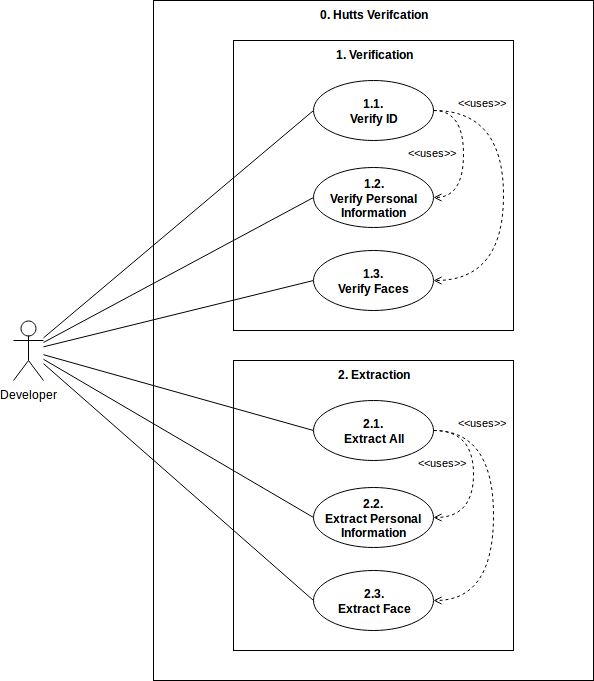
\includegraphics[scale=0.6]{img/use_case.png}
			\caption{Use Case Diagram for Hutts-Verification}
		\end{figure}
		\begin{enumerate}
			\item \underline{Verification Subsystem}
			\begin{enumerate}
				\item Verify ID
				\begin{enumerate}
					\item \textbf{Description:} The developer must be able to send a picture of an ID and the system should verify the ID against a photo of the individual in question. The personal information of the individual should also be verified.
					\item \textbf{Precondition:} Two photos with a high DPI and reasonable, proportionate lighting.
					\item \textbf{Postcondition:} The system verifies and returns a percentage match.
				\end{enumerate}
				\item Verify Personal Information
				\begin{enumerate}
					\item \textbf{Description:} The developer must be able to send a picture of an ID and the system should verify the ID against provided personal information of the individual in question.
					\item \textbf{Precondition:} Personal information of the person in question should be provided.
					\item \textbf{Postcondition:} The system verifies and returns a percentage match.
				\end{enumerate}
				\item Verify Faces
				\begin{enumerate}
					\item \textbf{Description:} The developer must be able to send a picture of an ID and the system should verify the ID against a photo of the individual in question.
					\item \textbf{Precondition:} Two photos with a high DPI and reasonable, proportionate lighting.
					\item \textbf{Postcondition:} The system verifies and returns a percentage match.
				\end{enumerate}
			\end{enumerate}
			\item \underline{Extraction Subsystem}
			\begin{enumerate}
				\item Extract All
				\begin{enumerate}
					\item \textbf{Description:} The system should be able to extract the relevant personal information, as well as the face of the person in the given ID.
					\item \textbf{Precondition:} An ID with a high DPI and reasonable, proportionate lighting should be provided.
					\item \textbf{Postcondition:} The system returns the extracted text and the extracted face.
				\end{enumerate}
				\item Extract Personal Information
				\begin{enumerate}
					\item \textbf{Description:} The system should be able to extract the relevant personal information from a photo of the ID document.
					\item \textbf{Precondition:} An ID with a high DPI and reasonable, proportionate lighting should be provided.
					\item \textbf{Postcondition:} The system returns the extracted text.
				\end{enumerate}
				\item Extract Face
				\begin{enumerate}
					\item \textbf{Description:} The system should be able to detect and extract the face of the person in the given ID.
					\item \textbf{Precondition:} An ID with a high DPI and reasonable proportionate lighting should be provided.
					\item \textbf{Postcondition:} The system returns the extracted face.
				\end{enumerate}
			\end{enumerate}
		\end{enumerate}
		\begin{table}[h]
\centering
\caption{Traceability Matrix}
\label{my-label}
\begin{tabular}{cc|c|c|c|c|c|l|l|l|l|l|l|l|}
\cline{3-14}
                                        &                   & \multicolumn{12}{c|}{\textbf{Functional Requirements}} \\ \hline
\multicolumn{1}{|c|}{\textbf{Use Case}} & \textbf{Priority} & 1 & 2 & 3 & 4 & 5  & 6 & 7 & 8 & 9  & 10 & 11 & 12 	 \\ \hline
\multicolumn{1}{|c|}{1.1}               & 6                 & X &   &   &   &    &   &   &   &    &    &    &    	 \\ \hline
\multicolumn{1}{|c|}{1.2}               & 4                 & X &   &   &   & X  &   & X & X & X  &    &    & X  	 \\ \hline
\multicolumn{1}{|c|}{1.3}               & 5                 & X &   &   &   &    & X &   & X &    &    &    & X  	 \\ \hline
\multicolumn{1}{|c|}{2.1}               & 3                 & X &   &   &   &    &   &   &   &    &    &    &    	 \\ \hline
\multicolumn{1}{|c|}{2.2}               & 1                 & X & X &   &   &    &   &   &   &    & X  & X  &    	 \\ \hline
\multicolumn{1}{|c|}{2.3}               & 2                 & X &   & X & X &    &   &   &   &    & X  & X  &    	 \\ \hline
\multicolumn{2}{|c|}{\textbf{Requirement Priority}}         & 1 & 5 & 4 & 6 & 10 & 8 & 7 & 3 & 11 & 2  & 12 & 9  	 \\ \hline
\end{tabular}
\end{table}
		
		
		
		\subsection{Performance Requirements}\label{subsec:specific-performance}
		\begin{itemize}
		\item A single extraction request should return in under 100 milliseconds.
		\item The system should be able to process 4 concurrent extraction requests in under 200 milliseconds.
		\item Any facial verification request should be handled in 5 seconds.
		    \item Any internal errors and exceptions should be handle by the system itself.
		\end{itemize}

		\subsection{Design Constraints}\label{subsec:specific-constraints}
		\begin{itemize}
		    \item The system will be implemented using Python 3.5 in order to ensure compatibility between the API and the Quant Solutions system.
		\end{itemize}

		\subsection{Software System Attributes}\label{subsec:specific-software}
		This section describes all quality related requirements
		\subsubsection{Reliability}
		\begin{enumerate}
		    \item The system should not fail when given a clear, well-lit photo of the identification document.
		    \item The system should always give a percentage match above the specfied threshold if the faces are the same.
		    \item Error handling should be implemented and the application should be able to handle all errors in a graceful manner by making use of helpful and descriptive error messages.
		\end{enumerate}
		\subsubsection{Security}
		\begin{enumerate}
		    \item All incoming and outgoing data will be encrypted using the HTTPS protocol due to the sensitive nature of the data collected.
		\end{enumerate}
		\subsubsection{Availability}

		\subsection{Other Requirements}\label{subsec:specific-other}
		\begin{itemize}
            \item Documentation should be of such a standard that anyone can easily implement the application when needed.
            \item The system should indicate that images match only if the images match with an accuracy of at least 75\%.
		\end{itemize}
		\section{Technology Choices}
		This section describes the technologies in use, and the
		arguments behind why we decided on these technologies.\\
		It was important to us to try and utilise technologies that are,
		free to use, efficient, relatively small in terms package size and
		requires as few as possible dependencies. 
		\subsection{
		\href{http://docs.opencv.org/3.0-beta/doc/py_tutorials/py_tutorials.html}			{OpenCV-Python Version \textit{3.2.0}}}
		OpenCV (Open Source Computer Vision Library) is free for commercial use.
		OpenCV is a well-documented and supported Computer Vision library
		since it has been available and been developed on for over 15 years at this point.
		OpenCV is available in many programming language 
		including Python, which was one of the requirements specified by the client.
		OpenCV now also supports multi-core hardware acceleration, which will
		increase efficiency drastically. \\
		
		\noindent
		OpenCV will be used for real-time processing of images throughout the system,
		which will include image clean-up image extraction and image manipulation.
	
		\subsection{\href{http://dlib.net/}{Dlib \textit{19.4.0}}}
		Dlib is an open source Machine learning toolkit and is also
		the only open source machine learning library that supports facial landmark
		optimisation and face likeness calculations out of the box.\\ 
		
		\noindent
		Dlib allows us to make use of a high quality, pre-trained classifiers
		for facial likeness, which made use of over 3 million faces 
		during training. This allows for an accuracy of 99.38 \%, according to the author of Dlib, in the
		\href{http://vis-www.cs.umass.edu/lfw/}
		{\textit{Labeled Faces in the Wild}}
		bench mark, thus allowing us to meet most of our performance requirements
		in terms of the face likeness calculations. \\
		
		\noindent
		Dlib also allows for face detection, as well as facial landmark 
		detection, both of which is required to improve the
		accuracy and reliability of the face likeness algorithm by supporting
		the alignment and clean-up of detected faces.
		
		\subsection{\href{https://pypi.python.org/pypi/pytesseract}
		{Pytesseract \textit{0.1.7}}}
		Python-tesseract is an open source optical 
		character recognition (OCR) tool for python. This allows 
		for the reading and decoding of embedded text in images.\\
		
		\noindent
		Tesseract allows for easy, automated scanning of cards. By making use
		of Tesseract we no longer need to:
		\begin{enumerate}
			\item Detect region of text.
			\item Process region of text.
			\item Use a trained classifier to read the extracted text.
		\end{enumerate}
		If it is found later to be a necessity in future, Tesseract supports
		additional training of fonts, which will allow for greater
		reliability and accuracy when extracting text.  
	
	\cleardoublepage

\end{document}
